\documentclass[a4paper,12pt]{article}
\usepackage[utf8]{inputenc}
\usepackage{graphicx}
\usepackage{amsmath}
\usepackage{amssymb}
\usepackage{hyperref}
\usepackage{caption}
\usepackage{subcaption}

\newcommand{\mb}[1]{\ensuremath{\mathbf{#1}}}
\newcommand{\mc}[1]{\ensuremath{\mathcal{#1}}}
\newcommand{\mbb}[1]{\ensuremath{\mathbb{#1}}}

%opening
\title{Second exercise assignment}
\author{Lucas Nogueira Ribeiro}
\date{}

\begin{document}

\maketitle

The Python source code written to solve this assignment is available at \url{https://github.com/lnribeiro/patternrecognition}.

\subsection*{Exercise \#01}
Consider a Bernoulli random variable $x \in \{0,1\}$ parametrized in $\mu$. Its probability density function is given by $p(x|\mu) = \mu^x(1-\mu)^{1-x}$.
\begin{itemize}
  \item The mean value of $x$ is given by \[\mathbb{E}[x] = \sum_{x\in\{0,1\}} xp(x|\mu) = 0.(1-\mu) + 1.\mu = \mu\]
  \item The variance of $x$ is given by \[var[x] = \mathbb{E}[x^2] - \mathbb{E}[x]^2 = \sum_{x\in\{0,1\}} xp(x|\mu) = 0^2.(1-\mu) + 1^2.\mu - \mu^2 = \mu(1-\mu)\]
\end{itemize}

\subsection*{Exercise \#02}
The covariance matrix of $\mb{X}$ is:
\begin{verbatim}
 [[  0.49866646  -0.10245845   0.4109965 ]
 [ -0.10245845   1.33957189   3.89705712]
 [  0.4109965    3.89705712  16.13133976]]
\end{verbatim}
By inspection, $var[x_1] = 0.498$, $var[x_2] = 1.339$, and $var[x_3]=16.13$. The variables pair $(x_1,x_2)$ is negatively correlated since $cov[x_1,x_2] = -0.10$. On the other hand, the pairs $(x_1,x_3)$ and $(x_2,x_3)$ are positively correlated since $cov[x_1,x_3] = 0.41$, and $cov[x_2,x_3] = 3.89$. The scatterplot diagrams of the random variables are depicted in Fig.~\ref{fig:scatter}. The mean values of the random variables are:
\begin{verbatim}
 mean(x_1): -0.000089
 mean(x_2): 0.111424
 mean(x_3): 0.160293
\end{verbatim}
It is not possible to infer the data probability distribution function (pdf) just by calculating its mean value and plotting its values. The histograms of the three random variables were calculated (using the builtin \verb|matplotlib.hist| Python module) to give us an idea of how they are distributed. Histograms \ref{fig:e22} and \ref{fig:e23} resembles Gaussian pdfs, whereas histogram \ref{fig:e21} presents spikes at $\pm 1$, similar to a arcsine pdf. 
\begin{figure}[t!]
    \centering
    \begin{subfigure}[t]{0.5\textwidth}
        \centering
        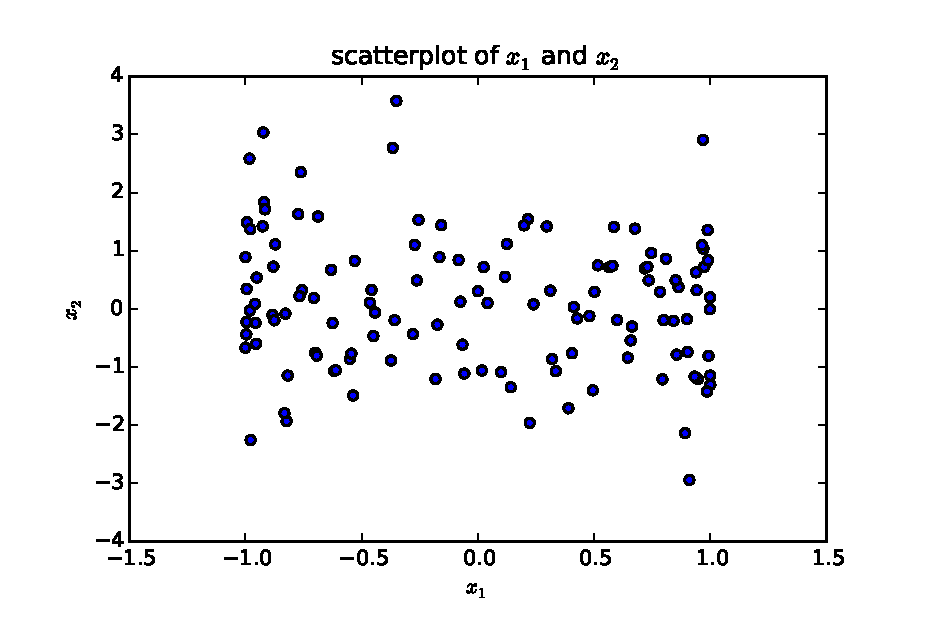
\includegraphics[height=2in]{figures/e2_scatter_x12.eps}
        \caption{Scatterplot of $x_1$ and $x_2$.}
    \end{subfigure}%
    ~  % same line
    \begin{subfigure}[t]{0.5\textwidth}
        \centering
        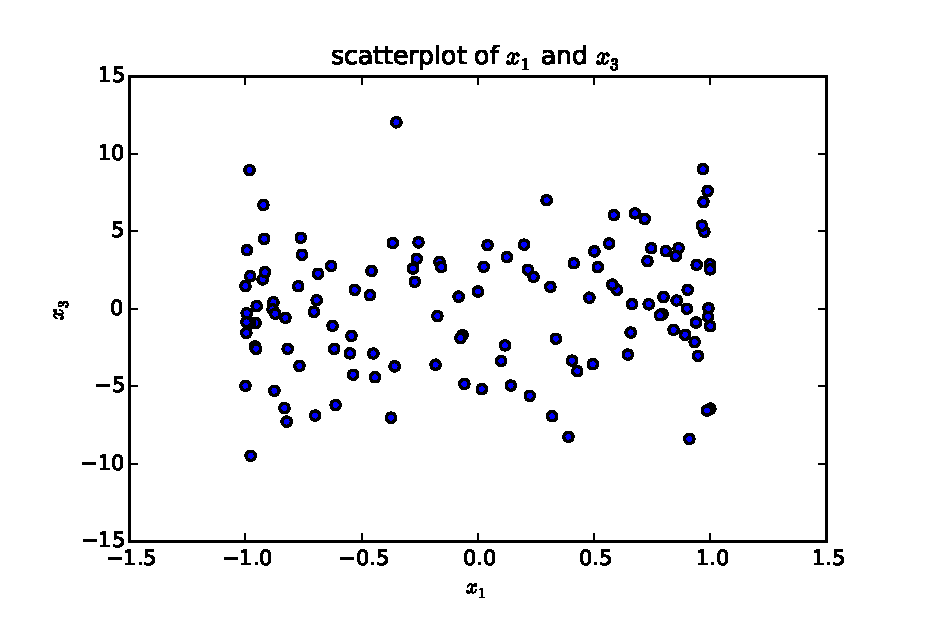
\includegraphics[height=2in]{figures/e2_scatter_x13.eps}
        \caption{Scatterplot of $x_1$ and $x_3$.}
    \end{subfigure}%
     %break line
     
    \begin{subfigure}[t]{0.5\textwidth}
        \centering
        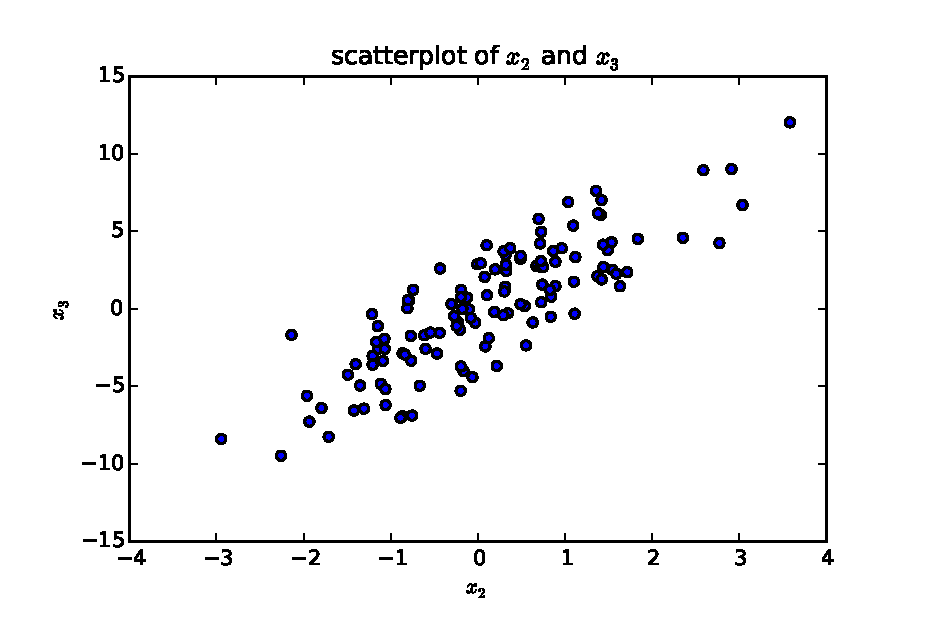
\includegraphics[height=2in]{figures/e2_scatter_x23.eps}
        \caption{Scatterplot of $x_2$ and $x_3$.}
    \end{subfigure}    
    \caption{Scatterplots of the generated data}
    \label{fig:scatter}
\end{figure}

\begin{figure}[t!]
    \centering
    \begin{subfigure}[t]{0.5\textwidth} 
        \centering
        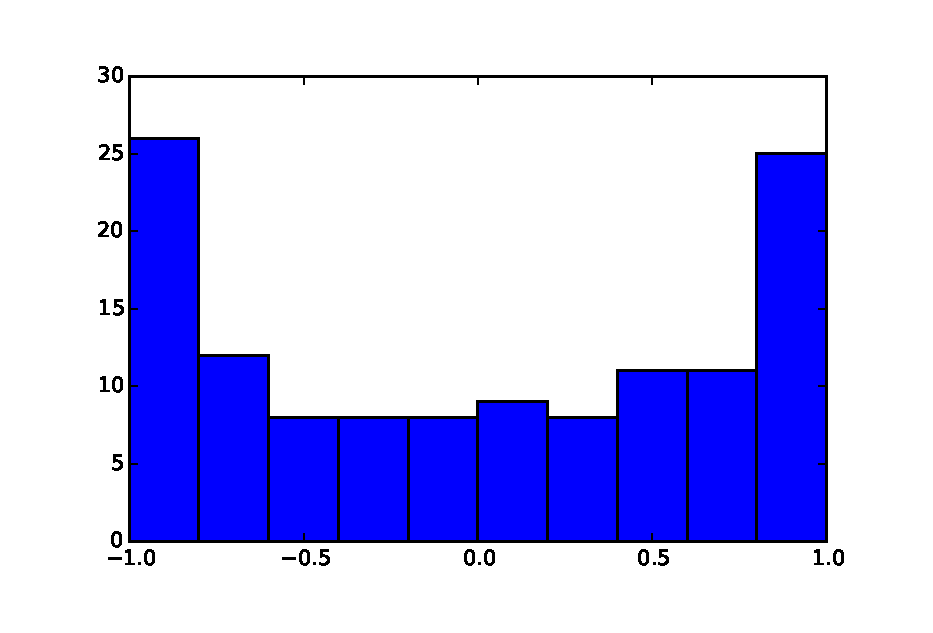
\includegraphics[height=2in]{figures/e2_hist_x1.eps}
        \caption{Histogram of $x_1$.}
        \label{fig:e21}
    \end{subfigure}%
    ~  % same line
    \begin{subfigure}[t]{0.5\textwidth}
        \centering
        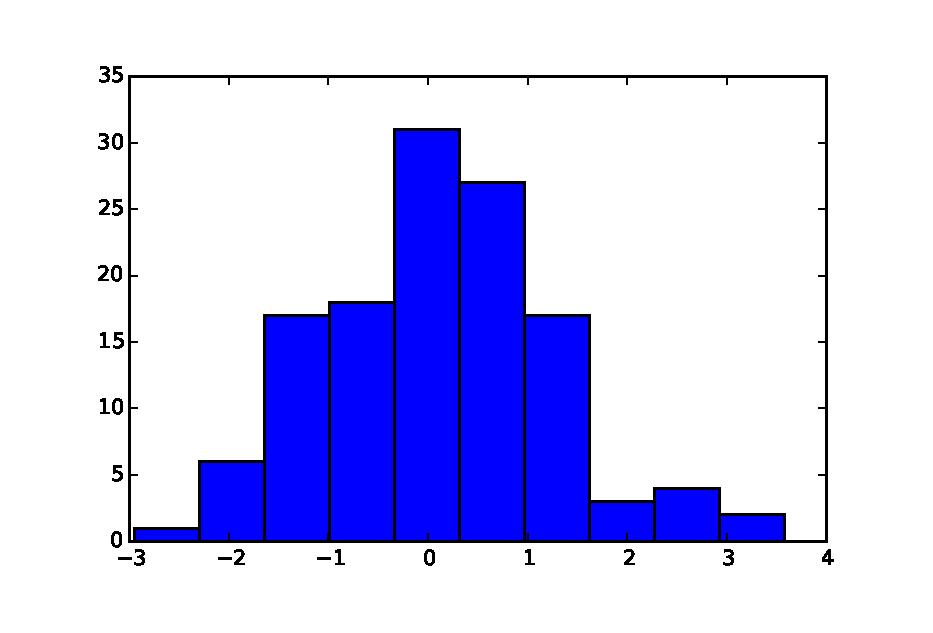
\includegraphics[height=2in]{figures/e2_hist_x2.eps}
        \caption{Histogram of $x_2$.}
        \label{fig:e22}
    \end{subfigure}%
     %break line
     
    \begin{subfigure}[t]{0.5\textwidth}
        \centering
        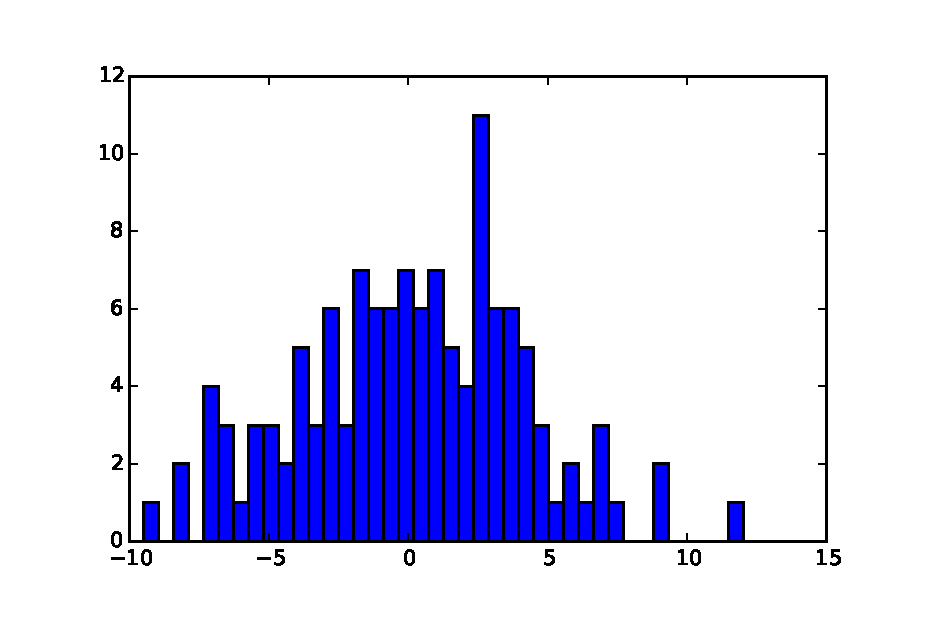
\includegraphics[height=2in]{figures/e2_hist_x3.eps}
        \caption{Histogram of $x_3$.}
        \label{fig:e23}
    \end{subfigure}    
    \caption{Histograms of the generated data}
    \label{fig:hist}
\end{figure}

\cleardoublepage
\subsection*{Exercise \#03}
The following histograms were generated using our own Python implementation. An intermediate value for $\Delta$, say 0.25, gives good results.
\begin{figure}[h]
    \centering
    \begin{subfigure}[t]{0.5\textwidth} 
        \centering
        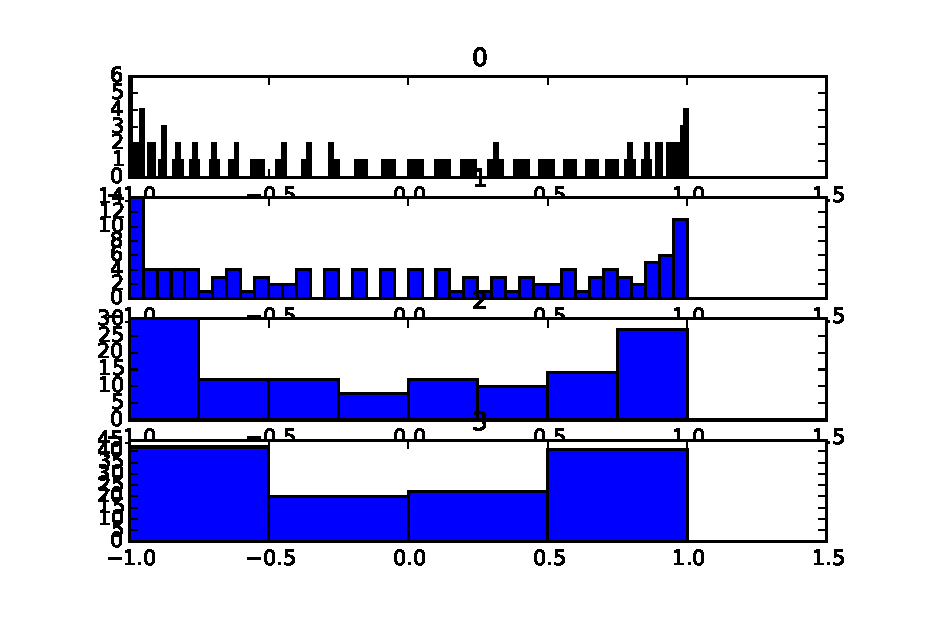
\includegraphics[height=2in]{figures/e3_hist_x1.eps}
        \caption{Histogram of $x_1$.}
        \label{fig:e21}
    \end{subfigure}%
    ~  % same line
    \begin{subfigure}[t]{0.5\textwidth}
        \centering
        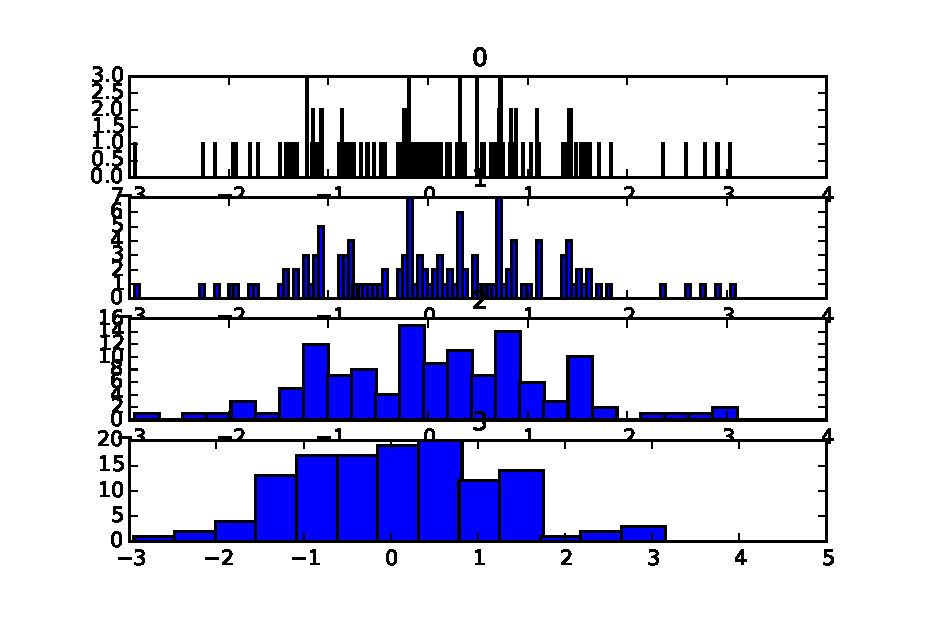
\includegraphics[height=2in]{figures/e3_hist_x2.eps}
        \caption{Histogram of $x_2$.}
        \label{fig:e22}
    \end{subfigure}%
     %break line
     
    \begin{subfigure}[t]{0.5\textwidth}
        \centering
        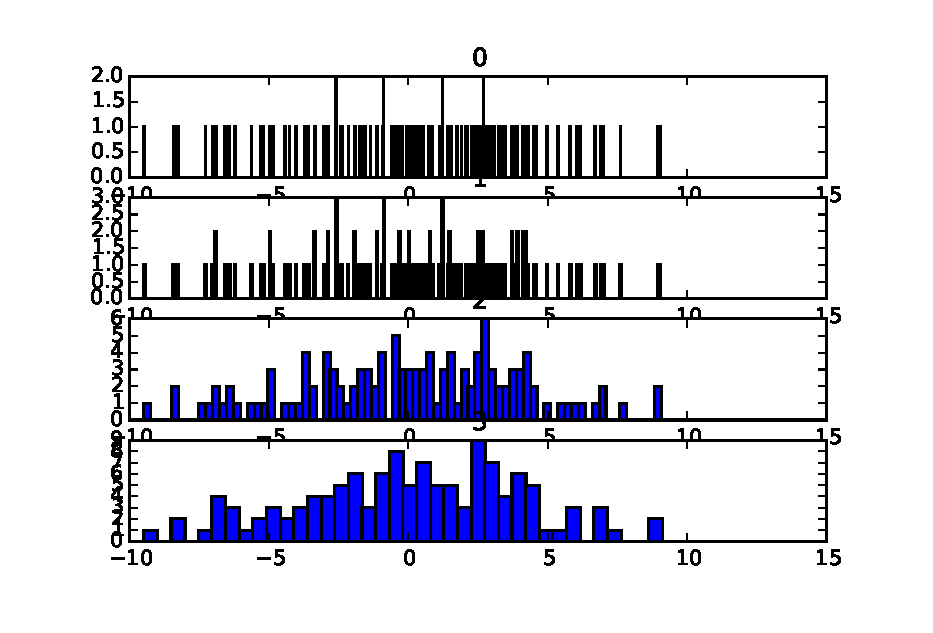
\includegraphics[height=2in]{figures/e3_hist_x3.eps}
        \caption{Histogram of $x_3$.}
        \label{fig:e23}
    \end{subfigure}    
    \caption{Histograms of the generated data using $\Delta=0.01, 0.05, 0.25, 0.5$.}
    \label{fig:hist}
\end{figure}

\cleardoublepage
\subsection*{Exercise \#04}
In this exercise, the $K$ nearest neighbors (kNN) was used to estimate the density function of $x_1$, $x_2$, and $x_3$. It consists of a nonparametric estimation method based on a neighborhood averaging. The estimated densities are depicted below.

\begin{figure}[h]
    \centering
    \begin{subfigure}[t]{0.5\textwidth} 
        \centering
        \includegraphics[height=2in]{figures/knn_x1_1.eps}
        \caption{$K=1$}
    \end{subfigure}%
    ~  % same line
    \begin{subfigure}[t]{0.5\textwidth}
        \centering
        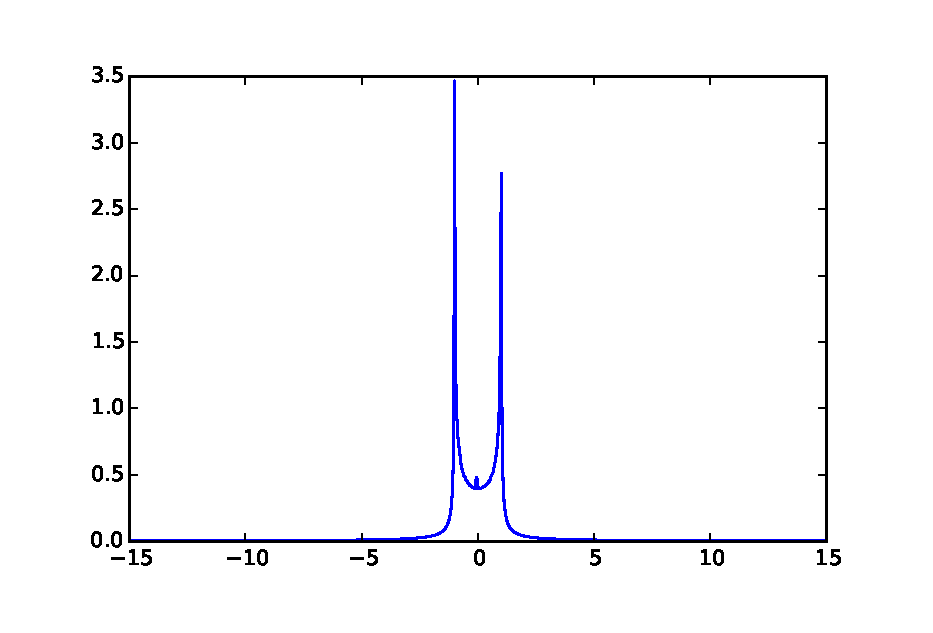
\includegraphics[height=2in]{figures/knn_x1_5.eps}
        \caption{$K=5$}
    \end{subfigure}%

    \begin{subfigure}[t]{0.5\textwidth}
        \centering
        \includegraphics[height=2in]{figures/knn_x1_10.eps}
        \caption{$K=10$}
    \end{subfigure}%
    ~
    \begin{subfigure}[t]{0.5\textwidth}
        \centering
        \includegraphics[height=2in]{figures/knn_x1_15.eps}
        \caption{$K=15$}
    \end{subfigure}    
    \caption{Estimated pdf of $x_1$ for different $K$.}
\end{figure}

\begin{figure}[h]
    \centering
    \begin{subfigure}[t]{0.5\textwidth} 
        \centering
        \includegraphics[height=2in]{figures/knn_x2_1.eps}
        \caption{$K=1$}
    \end{subfigure}%
    ~  % same line
    \begin{subfigure}[t]{0.5\textwidth}
        \centering
        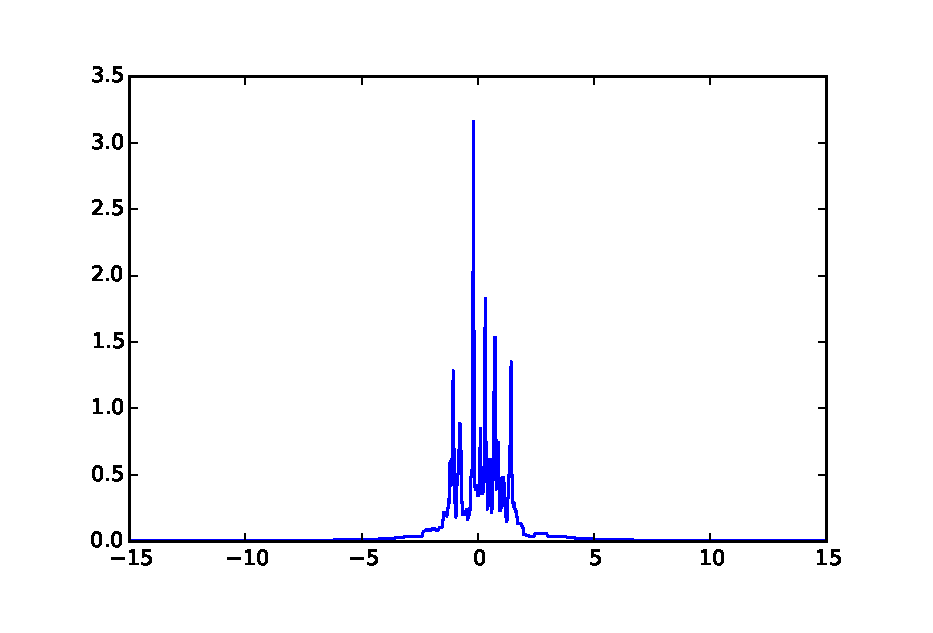
\includegraphics[height=2in]{figures/knn_x2_5.eps}
        \caption{$K=5$}
    \end{subfigure}%

    \begin{subfigure}[t]{0.5\textwidth}
        \centering
        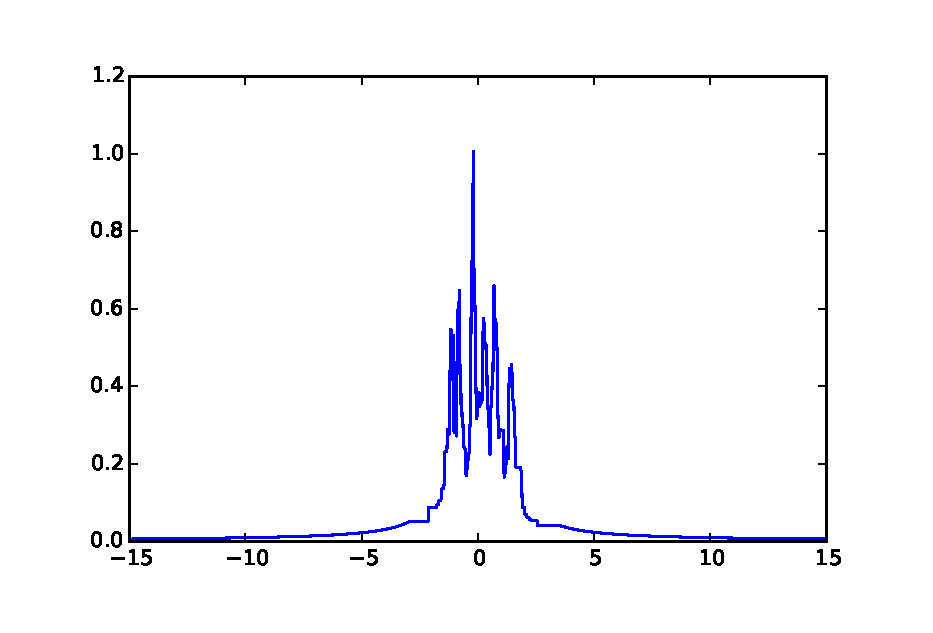
\includegraphics[height=2in]{figures/knn_x2_10.eps}
        \caption{$K=10$}
    \end{subfigure}%
    ~
    \begin{subfigure}[t]{0.5\textwidth}
        \centering
        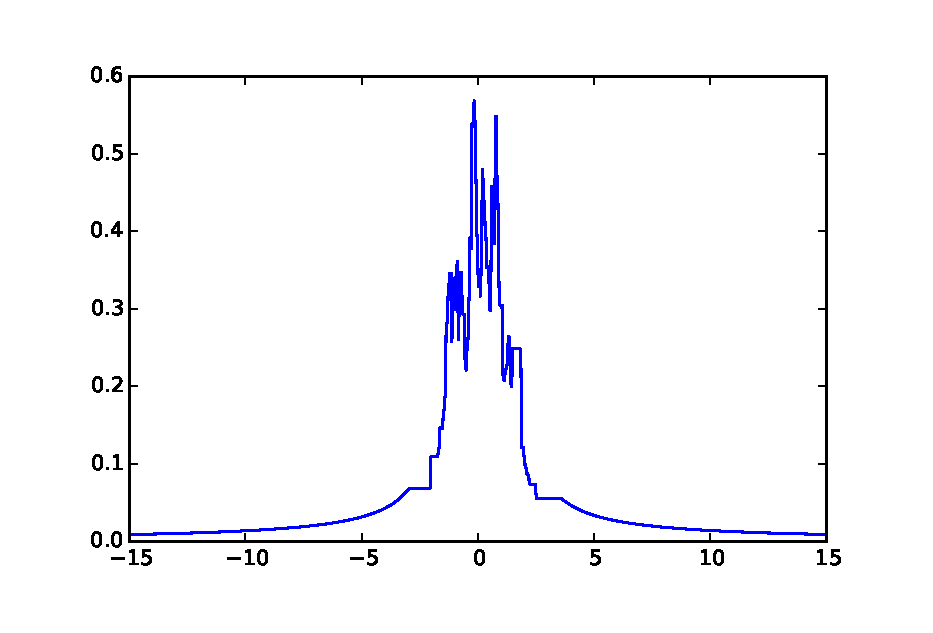
\includegraphics[height=2in]{figures/knn_x2_15.eps}
        \caption{$K=15$}
    \end{subfigure}    
    \caption{Estimated pdf of $x_2$ for different $K$.}
\end{figure}

\begin{figure}[h]
    \centering
    \begin{subfigure}[t]{0.5\textwidth} 
        \centering
        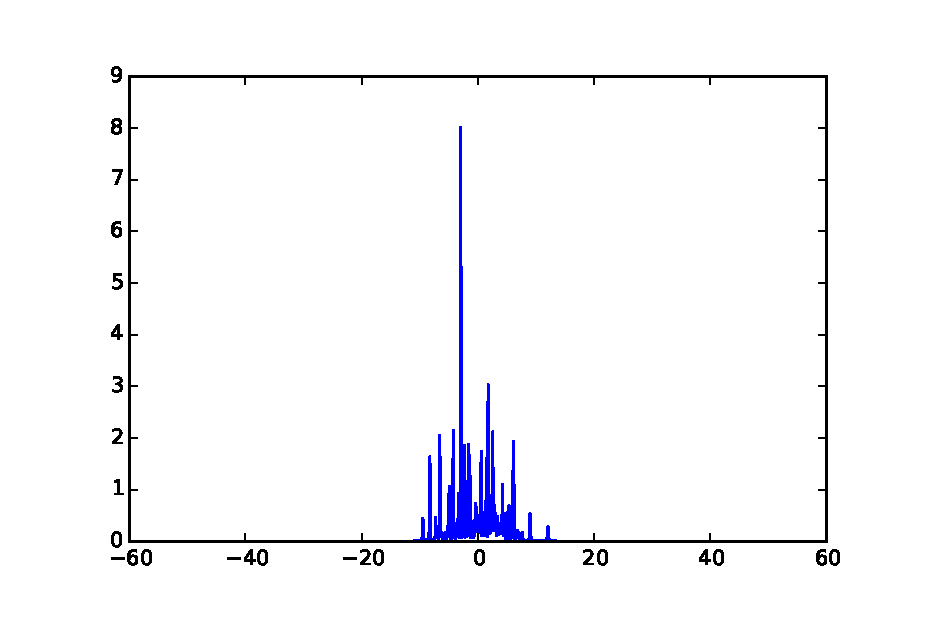
\includegraphics[height=2in]{figures/knn_x3_1.eps}
        \caption{$K=1$}
    \end{subfigure}%
    ~  % same line
    \begin{subfigure}[t]{0.5\textwidth}
        \centering
        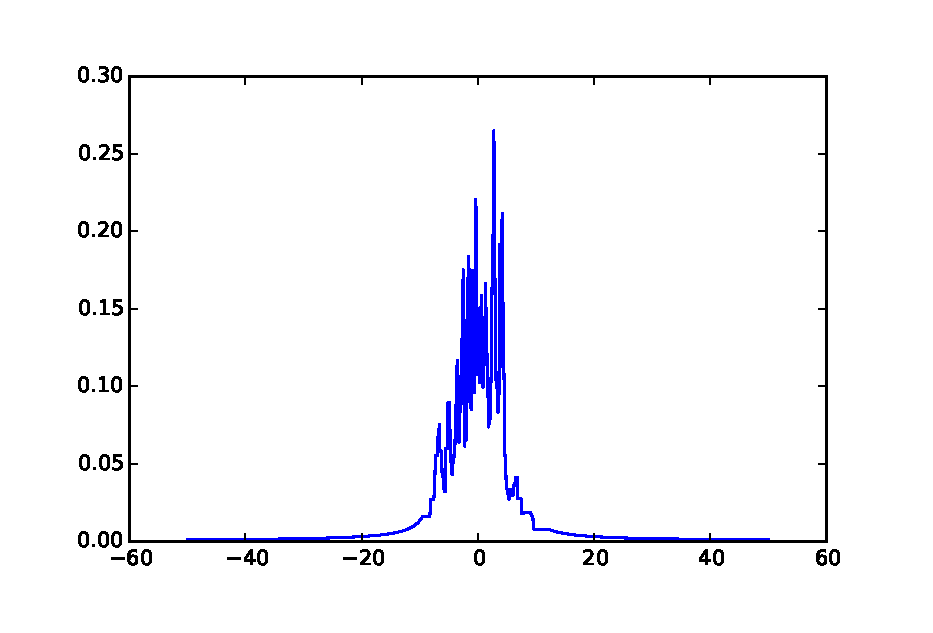
\includegraphics[height=2in]{figures/knn_x3_5.eps}
        \caption{$K=5$}
    \end{subfigure}%

    \begin{subfigure}[t]{0.5\textwidth}
        \centering
        \includegraphics[height=2in]{figures/knn_x3_10.eps}
        \caption{$K=10$}
    \end{subfigure}%
    ~
    \begin{subfigure}[t]{0.5\textwidth}
        \centering
        \includegraphics[height=2in]{figures/knn_x3_15.eps}
        \caption{$K=15$}
    \end{subfigure}    
    \caption{Estimated pdf of $x_3$ for different $K$.}
\end{figure}

\end{document}


